\chapter{Context-Dependent Environments: \\ A Parameterization Paradigm for Hardware Generators}
\label{c.parameters}

As Moore's law fails, increasing demand for computational efficiency is no longer being matched by gains from process scaling. 
Instead, chip designers are improving efficiency by combining special-purpose accelerators with general-purpose processors in increasingly heterogenous systems-on-chip.
In this new world of energy-efficient, heterogeneous, application-specific designs, it will be essential to both improve the productivity of hardware designers as well as enable extensive design-space exploration~\cite{shacham-micro10}.

Since it is not possible to build custom chips from scratch for every application,
we need hardware design tools that allow us to capture decisions made
during the process of designing one chip and easily make them differently when tackling a new target.
Creating parameterized hardware generators rather than individual design instances not only allows for application-specific customization of the final hardware,
but also gives designers the capability to preserve knowledge related to performance and energy trade-offs from previous design iterations.
By parameterizing aspects of the design, we can scale it from test chip sizes to final product without rewriting any modules, amortizing verification costs and increasing the validation confidence over time without rewriting code.
This templated, meta-programming approach is integral to our agile aproach to hardware design.

The most salient feature of a hardware generator or template, as
compared to a single design instance, is that certain features of the design are
left under the control of the user deploying the generator within their chip.
We term these features the {\em parameters} of the generator.
{\em Parameterization} is the process by which a generator supplies values for each parameter,
i.e. binds the name of the parameter to a particular value,
before using that evaluation to elaborate details of the particular design instance at hand.
A {\em parameterization paradigm} codifies a particular way of expressing parameters and provides tools to support their application within and injection into generators,
as well as mechanisms to constrain their valuations.

The parameters and their constraints become the interface through which the generator author and the system architect communicate.
Constrained parameters serve as boundaries that define the space of designs which it is possible for the architect to explore.
By searching over the top-level parameters exposed by a set of such generators, SoC chip architects can explore tradeoffs between performance, area, and energy efficiency.
By recording the outcomes of these explorations, these designers can build up a map of how to customize pieces of their design for a particular application's requirements.

Parameterization is clearly a first-order concern in the creation of tools based around specialized hardware generation.
In order to use generators productively, we need to understand how the choice of parameterization paradigm affects the design process.
We claim that the mechanism by which generator-based designs are parameterized can greatly influence three metrics of design robustness: reusability, composability, and modifiability.
We define these three metrics as follows:
\begin{description}
\item[Resuing] generators means that they can be instantiated in different hardware contexts with no internal source code changes, only differing parameterizations. Reusability amortizes verification overhead by reducing the number of lines of code used to create design instances.
\item[Composing] generators requires mechanisms to specify cross-generator parameter constraints and dependencies. Composability is mandatory to build up larger SoC designs consisting of multiple generators.
\item[Modifying] a generator by changing its parameters should not cause a cascade of changes throughout any nested modules which instantiate that generator's output. Modifiability is predicated on modularity in the code base, and avoiding technical debt in the face of changing generator capabilities.
\end{description}

This chapter first provides a background discussion of how the concepts of parameterization and meta-programming are intertwined, as well as how software languages have addressed parameterization in the past.
We then provide a taxonomy of extant parameterization paradigms found in previous hardware description languages, and evaluate them in terms of the above metrics.
To correct for their deficiencies, we introduce \emph{context-dependent environments}~(CDEs), a new parameterization paradigm.
In the CDE paradigm, a key-value dictionary containing parameter bindings is passed through a hardware module hierarchy, and the value returned for each parameter identifier can depend on other parameter values at that query's origin within the design.
As we will see in this chapter,
the dynamic nature of a CDE's scoping, coupled with its context-specific knowledge, 
serves to support generator reusability and composition, while also improving a generator's robustness to any external module hierarchy modifications.

We provide both a case study and a formal analysis of design robustness with respect to each of the parameterization paradigms in our taxonomy, and prove that CDEs are the most robust option.
We then provide examples of how our open-source Scala implementation of CDEs is used in various sub-components of our RocketChip SoC generator.
As we will see later in this thesis, even a design choice as complicated and pervasive as a multi-level cache coherence protocol can be made a tuneable design parameter when properly factored out from the rest of the design. 
By providing support for generating a family of protocols rather than one single protocol, my thesis has enabled us to iterate on protocol design as we scale up the size of the memory hierarchy across chip iterations.

\section{Background}
\label{sec:rel}

%Given a set of top-level configurations that supply value bindings for individual parameters, a generator can construct a vast number of different designs from a single piece of templated source code.
%Hardware generators are an increasingly popular paradigm; examples include Stanford's FPU generator~\cite{fpu}, Lawrence Berkeley National Lab's OpenSoC~\cite{opensoc}, and UC Berkeley's Rocket Chip Generator~\cite{rocket}.
%Bluespec provides AzureIP Libraries~\cite{azure} to give designers reusable components for use in custom generators. 
%Support for parameterization is a critical feature of the language in which the generator is written.

To provide context for our study of the applicability of various parameterization paradigms to hardware generation,
as well as to motivate the value of our new CDE paradigm,
we will first review two concepts at the heart of parameterization:
meta-programming and name binding.
Meta-progamming allows us to create parameterized hardware templates, into which values can be injected to make concrete design instances.
Name binding is the process by which parameter identifiers are associated with particular values.

\subsection{Meta-programming}

When we talk about creating libraries of hardware generators instead of design instances,
the underlying concept that our design tools need to support is meta-programming of hardware descriptions.
A meta-program is a program that generates or manipulates program code~\cite{templates}.
Specifically in the case of this thesis, Chisel~\cite{chisel} is a meta-programming language (that is itself embedded in a host languagage, Scala).
Using Chisel, we can describe parameterized templates for particular hardware modules as Scala classes.
Executing a Scala program that instantiates particular instances of these classes allows the Chisel compiler
to elaborate a concrete design instance in Verilog or some other target language.
Because Chisel is embedded in Scala, we can use the full capabilities of this modern software language to implement our generators.
This chapter will make the case that one of the most essential capabilities that this embedding has put at our disposal
is the ability to use Scala to parameterize our hardware descriptions,
be it through built-in language capabilities or through parameterization frameworks written in the host language.

Traditional hardware description languages have lacked the language features to support parameterization of configurable designs.
Section \ref{sec:tax} will discuss how specific existing parameterization paradigms in Verilog, VHDL, SystemVerilog and Bluespec SystemVerilog limit design modifiability and customizability.
However, because the outputs of our generators will be fully elaborated designs with parameter values  automatically embedded in them,
we can free generator authors from the constraints of the backend language with respect to choice of parameterization paradigm.
This approach also allows us to supply parameter bindings from external tools at hardware generation time.
There are several different times during the hardware elaboration process where we might decide to supply parameter values, and in particular this chapter will discuss tradeoffs between
binding parameters to values at generator compile-time as opposed to generator run-time.

How parameters are expressed and referenced within and among generators is another important design question.
From the perspective of the author of a hardware generator, it is impossible to know the full context in which the components created by their generator will be instantiated.
Their goal of the author of a hardware generator is to expose as many parameters as they possibly can to the user (e.g. an SoC architect),
while also recording any constraints the internals of the design put on those parameters' values.
Our parameterization paradigm must also accept constraints that are imposed by parent modules on their children, in the service of interoperability,
or by completely external tools, in the service of design space exploration.
Again, we are aided by the expressionality of the host language and the ability to connect with outside tools at hardware generation time.
Finally, while the parameters themselves are often merely instances of simple numeric or boolean types
depending on the nature of the meta-programming language we can also consider utilizing parameters that are bound to functions, user-defined objects
or other parameters.
As we will see, exploiting a host language's capability to use more complicated types in the parameterization framework
is an essential requirement for using it to support customizable cache coherence protocols.

Given the limitations of extant HDLs, adopting new ones with first class support for meta-programming (and thereby parameterization)
is critical to our hardware design methodology.
Chapter 3 of ~\cite{shacham2011chip} provides additional discussion of the 
parameterization advantages related to meta-programming
in the context of Genesis2, a next-generation HDL embedded in perl.
We include a comparison with Genesis2's perl-based dynamic parameterization paradigm in Section \ref{sec:env}.

\subsection{Name Binding and Scoping}

The opportunity presented by embedding Chisel in Scala inspired us to examine parameterization solutions that have been investigated in software contexts.
Fundamentally, parameterization is a name binding problem, in which a data or code entity must be bound to an identifying name.
In our case, generators express the hardware they elaborate in terms of the parameters' identifiers, and the framework is in charge of supplying the matching data
as the hardware is generated.
What data is supplied for a particular name depends on the scoping of the identifier, which might be handled lexically or dynamically.
Lisp languages were the first to explore tradeoffs between dynamic scoping and lexical scoping \cite{gordon}.

With lexical scoping, in order to bind a name to an entity we first search in the local function, then the scope in which this function was defined, and so on.
``Lexical'' in this case refers to the text of the source code itself.
Lexical scoping provides referential transparency, which is a boon for both the programmer and compiler.
By analyzing the source code, it is possible to determine at compile time whether or not a particular binding is within scope.
Unfortunately, bindings needed by deeply nested components must be explicitly threaded throughout the class or function hierarchy.

With dynamic scoping, we again search first in the local function, but then search the function that called this function, and so on up the call stack of the running program.
``Dynamic'' in this case refers to the fact that the call stack can be different every time a given function is called, and so the binding created for the variable can thereby differ as well.
Dynamic binding is useful as a substitute for globally-scoped variables, and is excellent for deep customization of nested subsystems.
In cases where the necessary bindings may radically change from program instance to program instance, dynamic binding allows us to only specify those bindings that we know this instance will use.
Unfortunately, in some cases programmer errors that could have been caught at compile time in a lexically-scoped system become runtime errors in a dynamically-scoped system.

While lexical binding is now the norm for most programming languages, many mechanisms have been developed to allow programmers to explicitly tie in dynamic binding benefits where they are useful.
These include special binding forms in most Lisp variants
(e.g. \code{fluid-let} in Scheme \cite{steele} and \code{parameterize} in Racket \cite{flatt2013racket}),
implicit parameters \cite{lewis2000implicit}, and the Reader monad of Haskell \cite{jones1995functional}.
While these approaches all focus on re-enabling the parameterization flexibility of dynamic binding in a more controlled manner, 
the context-dependent environments we propose here are actually a strictly more powerful mechanism than traditional dynamic binding. 
In general, taking advantage of later-binding solutions enables both more concise uniquification of elements of nested, heterogenous systems~\cite{shacham2011chip},
and also allows us to more robustly deal with modifications to the hierarchy of generated modules.
The following taxonomy illustrates how selectively deploying our dynamic scoping solution is the best fit for hardware generation
by contrasting it with several lexically-scoped solutions.

\section{Taxonomy of Parameterization Paradigms}
\label{sec:tax}

Before introducing context-dependent environments, we first define and contrast three existing parameterization paradigms: argument lists, structs, and dynamic environments.
We examine how these paradigms could be or have been used in hardware description languages and evaluate them in terms of a simple case study
in which we describe making modifications to a hierarchical hardware generator that is composed from multiple sub-generators.
The three paradigms we contrast in this section are:

\begin{description}
\item[Argument Lists.] The default lexical binding approach wherein all parameters are explicitly passed to the constructor function of each hardware module class.
\item[Structs.] A more sophisticated lexcical binding approach wherein user-defined datatypes are used to abstract away specific parameter binding sites.
\item[Environments.] A dynamic binding approach wherein an associative array of key-value pairs is used to supply parameter values at runtime.
\end{description}

We do not consider some other simple alternative parameterization solutions, such as a flat namespace of global constants, because such implementations lack composability and reuseability.
Firstly, without a mechanism to manage namespace collisions between different third-party generators, composing generators without having to modify their internals becomes impossible.
Secondly, without a mechanism that allows designers to override parameter values within certain subsets of the module hierarchy, creating heterogenous systems where the same genereator
produces differently parameterized output becomes impossible.
For these reasons we only contrast the aforementioned three paradigms, as they support both design goals in their own ways.

%TODOEach scheme preserves module modularity and reusability by expressing all parameters at the top level and only requesting necessary parameters. We evaluate each paradigm's robustness by adding parameters/modules and counting the number of top-level (TLCs), non-local (NLCs), or local (LCs) source code changes cascading from this initial modification.

We can evaluate the robustness of these parameterization paradigms by adding new parameters or inserting additional modules, and then examining the source code changes required to bring the new parameter binding into scope. 
We differentiate three types of source code changes.

\begin{description}
\item[Local changes (LCs)] are the initial insertion or appending of a module instantiation with a new parameter. 
\item[Top-level changes (TLCs)] are new parameter bindings performed at the root of the module hierarchy. 
\item[Non-local changes (NLCs)] are any additional changes required to pass a top-level parameter value (bound by a TLC) to the scope of a lower-level module instantiation (created by an LC). 
\end{description}

LCs and TLCs are simply inherent to instantiating a new parameterized module or adding a new parameter to an existing module.
The module using the parameter must be instantiated somewhere in the hierarchy (LC), and the parameter must be bound to a value
somewhere in that instantiation's scope (TLC).
In some cases additional LCs are needed to resolve conflicting parameter names at the location where the module is instantiated.

In contrast, NLCs only serve to bring a new parameter binding into scope for the new module instantiation,
or alternatively to correct a inter-module parameter reference that has been outdated by a module insertion.
We view being forced to manually make NLCs within our generators' source code as representative of
the brittleness of a particular parameterization paradigm in the face of changes to child generator interfaces
or module hierarchy depth.
In this way, NLCs are a form of technical debt imposed by the choice of parameterization framework on a hardware generator library.
According to our robustness metric, an ideal parameterization paradigm would eliminate all NLCs,
while simultaneously minimizing the number of LCs and TLCs needed to implement any given design modification.
In general, NLCs are the cost of deploying a paradigm dependent on lexical binding rather than dynamic binding.

%To maximize design modularity and reusability by first binding all parameter names at the top level of the module hierarchy and then requesting necessary parameter values within each module. 
%While default values could be supplied locally, any parameters used in inter-generator design space exploration must be exposed at the top level of each generator.

The following sections use examples written in Verilog-like pseudo-HDL code which elides non-parameter-related expressions.
Figure~\ref{fig:phdl} outlines the syntax for object declaration and instantiation in our pseudo-HDL.
In this pseudo-HDL, we assume every hardware module can be made into a templated hardware generator through the use of the additional \code{\#()} constructor parameter list.
Fields of that list (or fields of objects within the list) are the parameters of the generator/module in question.
Figure~\ref{fig:block} displays the block diagram organization of a set of nested hardware modules that we will use in our robustness case study.
We take a Tile generator that is hierarchically composed of Core, Cache and FPU generators, and investigate how making modifications to the parameters
of the leaf generators impacts the rest of the design, as expressed in our pseudo-HDL.

\begin{figure}
\centering
\begin{phdl}
struct S {f:Bool,g:Int}          // struct declaration
module A #(p1,p2,p3,p4,p5)(...): ... 
   // module declaration: parameters use 1st argument list #(p1,...)
   // other RTL constructs like IOs use 2nd argument list (elided)
module B #()(...):
  a = new S(true, 1)             // struct instantiation
  b = a.f                        // struct access
  myA = new A #(a,b,c,d,e)(...)  // module instantiation
\end{phdl} 
\caption{Syntax for object declaration and instantiation in our HDL pseudocode.}
\label{fig:phdl}
\end{figure}

\begin{figure}
\centering
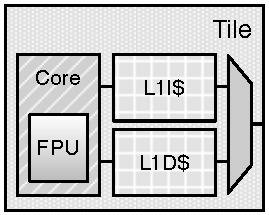
\epsfig{file=parameters/figures/tile.pdf, width=2.7in}
\caption{Organization of nested modules used in our running example.
A Tile contains one Core and multiple Caches.
A Core may or may not contain an FPU, which may or may not be parameterized.}
\label{fig:block}
\end{figure}

\subsection{Argument List Parameterization}

\begin{figure}
\centering
\begin{phdl}
module Top#()():
  hasFpu = true  // Whether our core should instantiate an FPU
  icSize = 64    // Size of the instruction cache's blocks
  dcSize = 64    // Size of the data cache's blocks
  myTile = new Tile #(hasFpu, icSize, dcSize)(...)
module Tile #(hasFpu, icSize, dcSize)(...):
  myCore = new Core  #(hasFpu)(...)
  icache = new Cache #(icSize)(...)
  dcache = new Cache #(dcSize)(...)
  assert (icSize == dcSize)         // The tile is multiplexing a single port
module Cache #(blockSize)(...): ... // icSize/dcSize each renamed blockSize
module Core #(hasFpu)(...):
  if(hasFpu) myFpu = new FPU()(...) ...
module FPU #()(...): ...
\end{phdl} 
\caption{An example module hierarchy containing a tile with a processor core and two caches, parameterized through constructor arguments.}
\label{fig:arglist}
\end{figure}

\begin{figure}
\centering
\begin{phdl}
module Top #()():
  hasFpu = true  // Whether our core should instantiate an FPU
  (*@\textcolor[rgb]{1,0,0}{fpuLat = 6}@*)     // Latency of FPU                               // TLC
  icSize = 64    // Size of the instruction cache's blocks
  dcSize = 64    // Size of the data cache's blocks
  myTile = new Tile #(hasFpu, icSize, dcSize,(*@\textcolor[rgb]{1,0,0}{fpuLat}@*))(...)        // NLC
module Tile #(hasFpu, icSize, dcSize,(*@\textcolor[rgb]{1,0,0}{fpuLat}@*))(...):               // NLC
  myCore = new Core  #(hasFpu, (*@\textcolor[rgb]{1,0,0}{fpuLat}@*))(...)                      // NLC
  icache = new Cache #(icSize)(...)
  dcache = new Cache #(dcSize)(...)
  assert (icSize == dcSize) 
module Cache #(blockSize)(...) : ... 
module Core #(hasFpu,(*@\textcolor[rgb]{1,0,0}{fpuLat}@*))(...) :                              // NLC
  if(hasFpu) myFpu = new (*@\textcolor[rgb]{1,0,0}{PFPU \#(fpuLat)}@*)(...) ...                 // LC
module PFPU #(latency)(...): ...     // Add parameter to FPU 
\end{phdl}
\caption{Example of the source changes required to append a new leaf submodule (PFPU) that contains a new parameter.}
\label{fig:arglist-delta}
\end{figure}

\emph{Argument list parameterization} is a paradigm wherein parameters are passed-by-value through class constructor function argument lists. 
It is the most basic, lexically-scoped way of binding parameters.
Verilog and VHDL are examples of existing HDLs that solely support this paradigm for parameterizing hardware modules.
 
Figure~\ref{fig:arglist} shows code describing the hierarchical \code{Tile} generator from Figure~\ref{fig:block} using argument list parameterization.
At the root of the module hierarchy, each parameter is bound to a value which is then passed into the module hierarchy via the argument list of \code{Tile}'s constructor.
These values are then propagated through the module hierarchy via the \code{Core} and \code{Cache} modules' constructors' argument lists.

In addition to injecting values into the design, we can enforce contraints on certain parameters.
For example, in this particular \code{Tile} architecture, both the instruction and data cache must have identical cache block sizes
because they are multiplexing the same memory port to the rest of the system.
This requirement is a property of this particular \code{Tile} generator; it was unknown to the designers of the \code{Cache} module.
Furthermore, other variations on a tile generator might not enforce this particular requirement, and so we would like to expose
\code{icSize} and \code{dcSize} to the design space explorer as independent, top-level variables.
Thus, the proper place to enforce the constrain is within \code{Tile}, making reference to the parameters that must be bound together.

Figure~\ref{fig:arglist-delta} illustrates how the argument list paradigm is brittle to modifications. 
We modify \code{Core} to use a parameterized FPU, \code{PFPU \#(fpuLatency)}, which takes as a parameter the desired latency for the unit.
In order to enact this modification, we must make several changes to the extant source code:
(1) a LC to instantiate the new \code{PFPU} within Core;
(2) a TLC to bind parameter \code{fpuLatency} in \code{Top};
(3) four NLCs to \code{Tile} and \code{Core}'s declaration parameter lists, as well as \code{Tile} and \code{Core}'s instantiations.
The four NLCs represent the brittleness of this particular paradigm, in that adding a parameter to a leaf module causes many non-local changes to be required in any interstitial modules.
For small designs with simple class hierarchies, the total number of NLCs might be small.
However, as we will see in Section~\ref{sec:scca}, in this paradigm the number of NLCs scales with module hierarchy size, making modifications increasingly burdensome
as the collection of generators in a particular lirbrary grows.

Further complexity arises if we consider a set of different FPU implementations, each with a unique or even partially overlapping set of parameters.
The set of parameters included in each intervening module's constructor becomes the superset of all the child modules' parameters.
Determining which parameters are actually unique and supplying default values for any which are unused in a particular design instance becomes onerous
as more and more combinations of generators are composed.

\subsection{Struct Parameterizations}

\begin{figure}
\centering
\begin{phdl}
struct TilePars {hasFpu:Bool, icSize:Int, dcSize:Int} // Structs definitions
struct CorePars {hasFpu:Bool}
module Top #()():
  tp = new TilePars(true, 64, 64)                     // Struct instantiation
  myTile = new Tile #(tp)(...)
module Tile #(params)(...):
  cp = new CorePars(params.hasFpu)                    // Struct instantiation
  myCore = new Core  #(cp)(...)
  icache = new Cache #(params.icSize)(...)
  dcache = new Cache #(params.dcSize)(...)
  assert (params.icSize < params.dcSize)
module Cache #(blockSize)(...) : ...
module Core #(params)(...):
  if(params.hasFpu) myFpu = new FPU()(...) ...
module FPU #()(...): ...
\end{phdl} 
\caption{The same example module hierarchy, but parameterized through flat structs instead of argument lists.}
\label{fig:flatstruct}
\end{figure}

\begin{figure}
\centering
\begin{phdl}
struct TilePars {hasFpu:Bool, icSize:Int, dcSize:Int, (*@\textcolor[rgb]{1,0,0}{fpuLat:Int}@*)} // NLC
struct CorePars {hasFpu:Bool, (*@\textcolor[rgb]{1,0,0}{fpuLat:Int}@*)}                         // NLC
module Top #()():
  tp = new TilePars(true, 64, 64, (*@\textcolor[rgb]{1,0,0}{6}@*))                              // TLC
  myTile = new Tile #(tp)(...)                                    // No NLC
module Tile #(params)(...):                                       // No NLC
  cp = new CorePars(params.hasFpu, (*@\textcolor[rgb]{1,0,0}{params.fpuLat}@*))                 // NLC
  myCore = new Core  #(cp)(...)                                   // No NLC
  icache = new Cache #(params.icSize)(...)
  dcache = new Cache #(params.dcSize)(...)
  assert (params.icSize < params.dcSize) ...
module Cache #(size)(...) : ...
module Core #(params)(...) :                                     // No NLC
  if(params.hasFpu) myFpu = new (*@\textcolor[rgb]{1,0,0}{PFPU \#(params.fpuLat)}@*)(...) ...   // LC
module PFPU #(latency)(...): ...     // Add parameter to FPU 
\end{phdl} 
\caption{Example of the source changes required to append a new leaf submodule (PFPU) that contains a new parameter,
under the flat-struct paradigm.}
\label{fig:flatstruct-delta}
\end{figure}

If the HDL provides user-defined struct types, these can be used to encapsulate multiple parameters within individual statically-typed objects.
SystemVerilog and Bluespec SystemVerilog are two HDLs that provide this capability.
For the purposes of our taxonomy, we posit that parameterization paradigms based on structs can be organized in two particular ways.
In \emph{flat-struct parameterization}, each generator is paired with a used-defined struct type containing all parameters used by that generator and all of its children.
This approach provides only a very limited advantage over the previously discussed argument list paradigm.
In \emph{nested-struct parameterization}, instead of a generator's companion struct consisting of a flat list of parameters,
it rather contains its own local parameters, as well as the parameter structs for its immediate children. 
This nesting allows further abstraction of the specific fields of the child generators' structs.

Both of these schemes are still lexically scoped, but we have moved the site of the bindings into a class hierarchy of struct types,
which may be distinct from the module hierarchy itself.
This level of indirection affords us, as generator authors, some opportunities to abstract away the specifics of what parameters are needed by which children.
By reducing the number of places we have to explicitly pass individual parameters' bindings from parent module to child module, we congruently reduce
the amount of work it takes to thread new parameters through the same module class hierarchy.
Encapsulation through structs can reduce the burden of lexical scoping in the face of design modifications.

Taking this idea a step further, we can recognize that we do not have to maintain a one-to-one mapping between the class hierarchy of structs and the class hierarchy of modules.
In the most extreme case, we could put all top-level parameters into a single struct which is passed to every module in the design,
essentially recreating a flat parameter paradigm based on global constants.
Such a solution improves modifiability by eliminating all NLCs, but is problematic for composability
because it means that sub-modules within the design cannot be reused in other contexts without providing default bindings for all possible parameters from all contexts.
However, more moderate solutions that exploit differences in the struct hierarchy and module hierarchy are possible at the designers' discretion.
For simplicity, the rest of this section utilizes the simpler one-to-one mapping to illustrate the differences between the struct paradigms.

Figure~\ref{fig:flatstruct} and Figure~\ref{fig:flatstruct-delta} show how the flat-struct paradigm,
applied with a one-to-one mapping between modules and structs,
can still eliminate some non-local changes in the face of appending the PFPU module as before.
This reduction is due to the fact that module constructor argument lists do not grow with additional parameters.
While the definitions of all the structs must be changed to account for the new parameter,
instances where a single struct instance is passed to multiple module instantiations do not need to be changed,
as the module instantiation no longer references the individual parameters, as they are now encapsulated fields of the struct.
However, Figure~\ref{fig:flatstruct-delta} shows that when inserting the newly parameterized \code{PFPU},
this scheme still requires some non-local changes because every parent generators's parameter struct declaration and instantiation must be changed.
In Section~\ref{sec:scca} we will see that the flat-struct paradigm is only a constant factor less brittle than the argument list paradigm.

\begin{figure}
\centering
\begin{phdl}
struct CorePars {hasFpu:Boolean, (*@\textcolor[rgb]{1,0,0}{fpuLat:Int}@*)}                     // NLC
struct TilePars {cp:CorePars, icSize:Int, dcSize:Int}            // No NLC
module Top #()():
  cp = new CorePars(true ,(*@\textcolor[rgb]{1,0,0}{fpuLat}@*))                                // TLC
  tp = new TilePars(cp, 64, 64)                                  // No NLC
  myTile = new Tile #(tp)(...)                                   // No NLC
module Tile #(params)(...):                                      // No NLC
  myCore = new Core  #(params.cp)(...)                                                        
  icache = new Cache #(params.icSize)(...)
  dcache = new Cache #(params.dcSize)(...)
  assert (params.icSize < params.dcSize) ...
module Cache #(size)(...): ...
module Core #(params)(...):                                     // No NLC
  if(params.hasFpu) myFpu = new (*@\textcolor[rgb]{1,0,0}{PFPU \#(params.fpuLat)}@*)(...) ...   // LC
module PFPU #(latency)(...): ...     // Add parameter to FPU 
\end{phdl} 
\caption{Example of the source changes required to append a new leaf submodule (PFPU) that contains a new parameter,
under the nested-struct paradigm.}
\label{fig:nestedstruct-append}
\end{figure}

\begin{figure}
\centering
\begin{phdl}
struct CorePars {hasFpu:Bool, fpuLat:Int}
struct TilePars {cp:CorePars, (*@\textcolor[rgb]{1,0,0}{cpf:CachePFPars}@*), dcSize:Int}      // NLC
struct CachePfPars {dist: Int, size:Int} // New struct for Prefetcher
module Top #()():
  (*@\textcolor[rgb]{1,0,0}{cpf = new CachePfPars(16, 64)}@*)  // Icache size now nested      // TLC
  cp = new CorePars(true, 6)
  tp = new TilePars(cp, (*@\textcolor[rgb]{1,0,0}{cpf}@*), 64)                                // NLC
  myTile = new Tile #(tp)(...)
module Tile #(params)(...):
  myCore = new Core  #(params.cp)(...)
  icache = new (*@\textcolor[rgb]{1,0,0}{CacheWithPF \#(params.cpf)(...)}@*)                   // LC
  dcache = new Cache #(params.dcSize)(...)
  assert ((*@\textcolor[rgb]{1,0,0}{params.cpf.size}@*) < params.dcSize)                      // NLC
module CacheWithPF #(params)(...):  // New module that adds prefetch functionality to cache
  myCache = new Cache #(params.size)(...)
... // Cache, Core, FPU declarations are unchanged
\end{phdl} 
\caption{Example of the source changes required to insert a new interstitial submodule (CacheWithPF) that contains a new parameter,
under the nested-struct paradigm.}
\label{fig::nestedstruct-insert}
\end{figure}

We can instead adopt \emph{nested-struct parameterization} to avoid the aforementioned cascading changes to all parent parameter structs' declarations and instantiations. 
Instead of a generator's companion struct consisting of a flat list of parameters, it contains only its own locally-consumed parameters as well as the parameter structs for its immediate children. 
Figure~\ref{fig:nestedstruct-append} applies this approach to the previous example of appending a parameterized FPU.
Only \code{PFPU}'s immediate parent's companion struct, \code{CorePars}, needs modification.
The fact that \code{CorePars} now has an additional parameter associated with it is now abstracted away from both \code{Tile} and \code{TilePars}.

Although the nested-structs paradigm eliminates almost all NLCs related {\em appending} new leaf modules to the hierarchy,
it retains another disadvantage related to {\em inserting} new levels into the module hierarchy.
Figure~\ref{fig:nestedstruct-insert} provides an example of a such a scenario.
Suppose we want to add a prefetcher to our instruction cache. 
We insert module \code{CacheWithPF}, with a single parameter (\code{distance}), that instantiates our original \code{Cache} module inside of itself.
\code{CacheWithPF} wraps \code{Cache}'s output with additional logic to perform prefecthing of expected instructions up to a specified \code{distance}.

The nested-struct paradigm does allow us to add \code{distance} without changing \code{Tile}'s constructor, avoiding an NLC.
Unfortunately, adding a new level of nesting in the parameter structs breaks our previously-existing assert statement in \code{Tile}. 
Because the nested structure of the parameter objects explicitly mirrors the generator hierarchy,
any changes to the nesting will break references to any child's parameters on which parent generators are enforcing constraints.
This results in a whole new class of NLCs to deal with, ones that could never have arisen with the simpler argument list approach!

While both struct paradigms are acceptable for flat class hierarchies with limited possible nestings,
generators often have deep module hierarchies or interoperate with other generators from multiple libraries
(correct interoperation often necessitates the imposition of constraints in parent generators).
These lexically-scoped paradigms embrittle such designs because changes to the module hierarchy break a parent's references to its childrens' parameters. 
Note that these broken references can be located anywhere in the design, often not located near the LC that inserts the new module.
Overall, even nested-structs cannot guarantee a robust design, despite significantly reducing NLCs related to appending new leaf modules.
Unsatisfied with lexical scoping for deeply nested generator hierarchies, we now turn our attention to dynamic scoping solutions.

\subsection{Environment Parameterization}
\label{sec:env}

\begin{figure}
\centering
\begin{phdl}
x = {'key1' -> 1,'key2' -> 3} // Environment instantiation
y = x ++ {'key1' -> 2}        // Environment modification
print x('key1')               // Environment query, prints '1'
print y('key1')               // Environment query, prints '2'
print y('key2')               // Environment query, prints '3'
\end{phdl}
\caption{Syntax for environment instantiation, modification and quering in our pseudo-HDL.}
\label{fig:env-phdl}
\end{figure}

\begin{figure}
\centering
\begin{phdl}
module Top #()():
  topPars = {'hasFpu'->true, 'icSize'->64, 'dcSize'->64} // Top-level bindings
  myTile = #(topPars)(...)
module Tile #(params)(...):
  myCore = new Core  #(params)(...)
  icache = Cache #(params('icSize'))(...)          // Parameter lookup
  dcache = Cache #(params('dcSize'))(...)          // Parameter lookup
  assert (params('icSize') < params('dcSize')) ... // Parameter lookups
module Cache #(size)(...) : ...
module Core  #(params)(...) :
  if(params('hasFpu') myFPU = new FPU #()(...) ... // Parameter lookup
\end{phdl} 
\caption{The same example module hierarchy, but parameterized through dynamic environments.}
\label{fig:env}
\end{figure}

\begin{figure}
\centering
\begin{phdl}
module Top #()():
  topPars = {'hasFpu' -> true, 'icSize' -> 64, 'dcSize' -> 64, (*@\textcolor[rgb]{0.8,0,0}{'fpuLat' -> 6}@*), (*@\textcolor[rgb]{1,0,0}{'dist' -> 16}@*) } // TLCs
  myTile = Tile #(topPars)(...)                                  // No NLC
module Tile #(params)(...):                                      // No NLC
  myCore = Core #(params)(...)                                   // No NLC
  // The following rename from `icSize' to `size' must be handled here by icache's parent
  (*@\textcolor[rgb]{1,0,0}{icPars = params ++ \{'size' -> params(`icSize')\}}@*)                // LC for CacheWithPF
  icache = new (*@\textcolor[rgb]{1,0,0}{CacheWithPF \#(icPars)(...)}@*)                        // LC for CacheWithPF
  dcache = new Cache #(params('dcSize'))(...)
  assert (params('icSize') < params('dcSize')) ...
module CacheWithPF #(params)(...) :
  Cache #(params('size'))(...) ... // CacheWithPF queries 'size'
module Core #(params)(...) :
   if(params('hasFpu') myFPU = new (*@\textcolor[rgb]{.8,0,0}{PFPU \#(params('fpuLat'))}@*)(...) // LC for PFPU
... // Cache, PFPU module declarations are unchanged
\end{phdl} 
\caption{Simultaneously appending a new submodule that contains a new parameter, while also inserting
a new interstitial module that contains a new parameter. Dynamic environments eliminate NLCs.}
\label{fig:env-delta}
\end{figure}

We begin by characterizing an environment-based approach to dynamic scoping of parameters.
An \emph{environment} is an associative array (i.e. map, dictionary), where each key and value pair consists of a parameter identifier and value respectively.
Environments can be inherited by an instance of a module and then passed along to its children, possibly
with modifications made to the key-value bindings.
Code within modules can gain access to certain parameter values by looking up the parameter's key in the environment.

Environments are a dynamic scoping solution because the value returned for each key is determined based on the execution of the program,
not the hierarchy of the source classes.
As alluded to earlier in this chapter, there are some tradeoffs inherent to dynamism.
Critically for composability, we do not have to pass bindings for all possible parameters through the module hierarchy explicitly.
This is a great boon for generators where some parameters are only used if certain other parameters are set a particular way,
or in cases where homogenous designs may be uniqueified to form heterogenous ones.
If a particular instance of a design does not use a particular parameter, that parameter never has to be bound.
If a new module is added, bindings for its parameters can be supplied to the environment from any parent location in the heirarchy.
The cost we pay for this flexibility is that unbound parameters can only be detected at runtime, rather than at compile time.

A popular use of dynamic environments in the software world are those used for processes in all flavors of Unix.
Whereas shell languages in Unix systems have a first-class syntax for accessing environment values (e.g. \code{\$HOME}),
attempts to implement environments in a previously existing HDL would have to explicitly pass the environment object through the module hierarchy to query it.
Unfortunately, SystemVerilog and BluespecSV (as well as Verilog and VHDL) cannot support environments, as environments require either nested functions or HashMaps.
While the SystemVerilog language includes associative arrays (similar to HashMaps), most SystemVerilog compilers do not support this language construct. 
This type of environment could be implemented in Bluespec or SystemVerilog using tagged unions or associative arrays.
Unfortunately, neither language supports dynamically typed parameters, and thus cannot pass associative arrays as parameter objects.
Bluespec requires all type checking be resolved prior to elaboration; since the compiler cannot guarantee that the returned value is type safe, associative arrays are not supported. 
Tagged unions, however, can be statically-type safe and used if the types of all parameters are known.
While both BluespecSV and SystemVerilog claim support for tagged unions, many SystemVerilog compilers lack support for them.

Chisel and Genesis2 leverage Scala and Perl, respectively, for metaprogramming the module hierarchy generation stage of hardware elaboration.
Because Scala and Perl support first-class functions and maps, both HDLs can easily provide the type of environment discussed here using either.
As we will see in Section~\ref{sec:impl}, Scala's support for implicit parameters makes it syntactically concise to distribute
the environment object through the module hierarchy.
Perl allows the programmer to select whether a variable is a dynamic global variable or a lexically-scoped local variable.
Rather than depend on the functionality global Perl environment, Genesis2 defines its own parameter environment framework that provides additional features.

Genesis2 supplies a parameter environment for each module and provides an API that allows users to:
define parameters,
assign them default values,
override those values from external configuration files,
force parameters to always take certain values,
and
define additional parameters at module instantiation time
\cite{shacham2011chip}.
A module can use a reference to any other module to make a reference to that module's parameters' values. 
Parameters are read-only, and queries return deep copies of mutable objects.
Because Perl is a dynamically-typed language, no type checking can be done on the return type of parameter queries.
The framework outputs XML to encapsulate the full ``configuration'', meaning the text description of how SystemVerilog module declarations are composed,
and allow for iterative customization of certain parameters values within the design in accordance with the experimental desing of external tools.
%Would need to explicitly rename parameters, can do this in multiple ways, including defining synonyms or referencing a parent's parameter. Adding parameters does require explicit renaming, no mechanism to reference child. Adding cde's would only benefit it, I think.

Figure~\ref{fig:env-phdl} provides an oveview of the additional syntax we introduce to our pseudo-HDL in order to allow it to support instantiation, modification, and querying of environments.
An important note is that the \code{++} operator, which adds a binding to the store, returns a new environment and does not affect the original environment.
In addition, all values in key-value pairs are lazily evaluated only when a query matches on a particular key.

Figure~\ref{fig:env} shows the code for our running example of the tile generator, modified to use the environment to supply parameters to all modules with two or more parameters.
To parameterize a child module, a parent copies its own environment and adds/overwrites any needed key-value mappings before passing it to the child.
While keys can be overridden in certain sub-modules, the overall namespace provided by the environment is flat, and does not codify anything about the structure of the module hierarchy.
Figure~\ref{fig:env-delta} demonstrates the advantages of this flexiblity by applying both of the modifications from previous case study examples
(replacing the appended \code{FPU} with \code{PFPU} and inserting \code{CacheWithPF}).
Significantly, the only changes required are LCs and TLCs, with no NLCs whatsoever.
Even the cross-module assertion on cache sizes in \code{Tile} does not require modification.

Although the environment passing paradigm succeeds in removing all NLCs,
there is an additional LC required to rename the \code{icSize} parameter to \code{size}.
Why does \code{CacheWithPF} query for \code{size} instead of \code{icSize}?
The generator designer wanted it to be composable with any cache, not bind it to a particular instance.
We should not contextualize the parameter name (e.g. change \code{size} to \code{icSize}) because the sub-module that is instantiated, in a different design, could be a data cache. 
Thus, an explicit renaming step is necessary to customize the parameter environment passed to \code{CacheWithPF}, telling it which top-level parameter to use
in response to any internal queries made regarding \code{size}.
We consider the source code change required to perform the renaming by modifying the environment an LC rather than an NLC because it always occurs in conjunction
with the LC that instantiates the newly inserted module.
However, it is worth noting that the renaming must be performed for each unique instance of the module that takes on a different, heterogeneous value.

In general, we will often have modules that have either intentionally picked a context-free key, or simply use parameter keys that coincidentally overlap with those
used by some other imported generator.
Differentiating these conflicting keys and assigning them to the proper top-level key bindings is both the power and the burden of the dynamic environment paradigm.
For designs that do not have a large number of parameter key collisions, environment passing is a great solution as it will significantly reduce the number of NLCs. 
Unfortunately, in the not uncommon case of designs that have many instances of the same child module class (e.g. a mesh of routers), the re-mapping of unique top-level parameters onto generic, re-used child parameters
that must occur every time one of these children is instantiatied becomes onerous.
To mitigate this burden through the use of geographic information, we now turn to context-dependent environments.

\section{Context-Dependent Environments}
\label{sec:cde}

\begin{figure}
\centering
\begin{phdl}
module Example :
  env1 = {'whoami' -> (*@\textcolor[rgb]{1,0.5,0}{\textbf{\textit{site}}}@*)('coord')}                // CDE instantiation
  env2 = env1 ++ {'coord' -> 'environment 2'} // CDE modification
  print env1('whoami')                        // CDE query, prints 'Error: 'coord' is not defined'
  print env2('whoami')                        // CDE query, prints 'environment 2'
\end{phdl}
\caption{Syntax for CDE instantiation and querying in our pseudo-HDL.}
\label{fig:cde-phdl}
\end{figure}

\begin{figure}
\centering
\begin{phdl}
module Top #()():
  constPars = { 'coefficient' -> 4 }                               // Constant function
  indexPars = { 'coefficient' -> List(4,5,6,7).at((*@\textcolor[rgb]{1,0.5,0}{\textbf{\textit{site}}}@*)('index')) } // Function on 'index'
  myHomogenousDSP   = new DSP4MultArray(constPars)     // Makes a DSP with identical coefficients
  myHeterogenousDSP = new DSP4MultArray(indexPars)     // Makes a DSP with unique coefficients
module DSP4MultArray #(params)(...):
  mult0 = new Mult #(params ++ {'index' -> 0}) m0(...) // DSP4MultArray provides context
  mult1 = new Mult #(params ++ {'index' -> 1}) m1(...)
  mult2 = new Mult #(params ++ {'index' -> 2}) m2(...)
  mult3 = new Mult #(params ++ {'index' -> 3}) m3(...) ...
module Mult #(params)(...):
  c = params('coefficient') ...                        // Mult only knows about coefficient, not index
\end{phdl}
\caption{Example of specifying geographic information using site in pseudo-HDL.}
\label{fig:site-phdl}
\end{figure}

We now describe the functionality of our novel context-dependent environments paradigm for parameterization,
and assess its robustness using the case study introduced in the previous section.
In the CDE paradigm, we again pass an associative array called an environment through a hardware module hierarchy, but the environment itself has an additional capability:
the value returned for a query on a key can depend on other parameter values at that query's origin within the design.
This feature is deceptively simple; the level of additional indirection provided in a CDE is a powerful tool for describing
parameters in terms of one another, which aids us in cascading uniquifying changes through subsets of a heterogeneous design.

While we previously demonstrated how we can use environments to provide the flexibility of dynamic binding on-demand from within a lexically-scoped module hierarchy, 
the CDEs we propose here are actually a strictly more powerful mechanism than traditional dynamic binding. 
We owe this power boost to our decoupling of ``how'' and ``when'' to compute a parameter's value,
allowing the ``how'' to be specified at binding time,
but deferring evaluation until the time at which the parameter is actually queried during elaboration.
This ``lazy'' evaluation strategy permits more parameter bindings to be in scope at
evaluation time than were available at binding time,
with the advantage that these other parameters may come from code locations not visible to the original binding site.

Mechanically, the sole additional feature of a CDE over a regular environment is a special object, called \emph{site}, that dynamically points to the originating CDE of the parameter query.
\emph{site} is available to be queried when defining the value bound to a particular identifier.
In other words, environment values bound within the environment are no longer mere literals, instead
they have been promoted to functions which take as an argument a dictionary representing the view of the world as seen from the query's point of origin.
When the environment is asked to evaluate a particular parameter identifier, the function stored for that key in the dictionary is evaluated against the dictionary itself.
Regular style environment variables are still possible in this paradigm, but now are just functions that ignore the dictionary argument and return a constant value (i.e. constant functions). 
We call these enhanced environments {\em context-dependent} because the valuations taken by their bindings depend on where the query is made.

\begin{figure}
\centering
\begin{phdl}
module Top #()() :
  topPars = {'hasFpu' -> true,
             'size' -> if((*@\textcolor[rgb]{1,0.5,0}{\textbf{\textit{site}}}@*)('loc') == 'iCache') 64 else 64 }
  myTile = new Tile #(topPars)(...)
module Tile #(params)(...):
  myCore = new Core #(params)(...)
  icache = new Cache #(params ++ {'loc' -> 'iCache'})(...) // Insert geographic location
  dcache = new Cache #(params ++ {'loc' -> 'dCache'})(...) // Insert geographic location
  assert (icPar('size') < dcPar('size')) ...
module Cache #(params)(...):
  ... params('size') ... // Cache queries CDE directly
module Core #(params)(...):
  if(params('hasFpu') myFpu = new FPU()(...) ...
\end{phdl} 
\caption{The same example module hierarchy, but parameterized through context-dependent environments.}
\label{fig:cde}
\end{figure}

\begin{figure}
\centering
\begin{phdl}
module Top :
  topPars = {'hasFpu' -> true,
             (*@\textcolor[rgb]{1,0,0}{'dist' -> 16}@*),                                   // TLC
             (*@\textcolor[rgb]{1,0,0}{'fpuLat' -> 6}@*),                                  // TLC
             'size' -> if((*@\textcolor[rgb]{1,0.5,0}{\textbf{\textit{site}}}@*)('loc') == 'iCache') 64 else 64 }
  myTile = new Tile #(topPars)(...)
module Tile (params)(...):
  myCore = new Core #(params)(...)
  icPar = params ++ {'loc' -> 'iCache'}                                                           
  icache = new (*@\textcolor[rgb]{1,0,0}{CacheWithPF}@*) #(params ++ {'loc' -> 'iCache'})(...) // LC
  dcache = new Cache #(params ++ {'loc' -> 'dCache'})(...)
  assert (icPar('size') < dcPar('size')) ...
module Cache #(params)(...):
  ... params('size') ...
module CacheWithPF (params)(...):
  Cache #(params)(...)        // CacheWithPF simply passes CDE
module Core (params)(...) :
  if(params('hasFpu') myFpu = new (*@\textcolor[rgb]{1,0,0}{PFPU \#(params)}@*)(...) // Core simply passes CDE  // LC
\end{phdl} 
\caption{Simultaneously appending a new submodule that contains a new parameter, while also inserting
a new interstitial module that contains a new parameter. Dynamic environments eliminate NLCs.}
\label{fig:cde-delta}
\end{figure}

Figure~\ref{fig:cde-phdl} provides a basic example of syntax and behavior for using the CDE {\em site} functionality in our pseudo-HDL.
We can see that \code{env1} is queried with the key \code{'whoami'}. 
This key is contained within \code{env1}, and its value, \code{site('coord')}, is evaluated. 
Because the original queried object is \code{env1}, \code{site} points to \code{env1} (i.e. \code{site('coord') == env1('coord')}). 
Since \code{env1} does not contain the key \code{'coord'}, this query fails.
The second query, \code{env2('whoami')}, matches because \code{env2} contains a \code{'whoami'} key. 
When \code{'whoami'}'s value is evaluated, \code{site('coord')} now points to \code{env2} (i.e. \code{site('coord') == env2('coord')}). 
Because \code{env2} contains a \code{'coord'} key, \code{site(`coord')} returns \code{'environment 2'}. 
This return value is propagated back to the original \code{env2('whoami')} callee and printed.

Now that every value in the environment can actually be a function of the bindings in the environment that is evaluating it, we can trivially
build meta-parameters that are based on formulae consisting of existing parameters, e.g. \code{\{"area"~->~site("length")~*~site("width")\}}.
This is a powerful capability for forming chains of parameter dependencies, in which parameters can be derived from other parameters.
Most importantly, these valuations can include reference to other parameters keys which were not known to the original generator authors,
but which are instead being defined by other generators in the hierarchy.
For example, while the original author of the \code{"area"} key may have specified only that it returns an interger,
composition with a Circle generator would override it to be bound to \code{\{"area"~->~pi~*~site("radius")~*~site("radius")\}}, whereas
composition with a Square generator would override it to be bound to the above example.
Furthermore, the actual bindings for \code{"width"}, \code{"length"}, or \code{"radius"} do not have to be supplied at the same time that
the meta-parameter \code{"area"} is bound to its value function.
As long as any interstitial generator binds those keys before the generator that uses \code{"area"} actually evaluates its query on that key,
everything will dynamically resolve to the correct value.

This \emph{site} functionality is particularly useful in the context of hardware generation because 
it allows for specialization of parameter values based on contextual or ``geographic'' information that was injected into the enviroment by any intermediate generator in the module hierarchy.
This capability is at the heart of how we uniquify modules in a heterogenous design.
Exploiting this capability requires that modules in a generator library built around the CDE paradigm follow the practice of placing geographic information
as new parameters in the environments they produce for their child modules, at the point where such geographic distinctions are clear. 
For instance, a network generator will instantiate and wire together the output of many router generators.
We would like a convenient way to assign different parameter values to the routers based on their location in the topology.
To achieve this effect, we place the burden on the parent (network) to append each child (router)'s inherited CDE with a constant parameter, e.g. \code{\{"location"~->~(x, y)\}}.
Assuming this geographic information will be inserted into the environment by the parent,
the top-level environment is free to tune each router's behavior according to \code{"location"}
by referencing it in the site-based function \code{\{"route"~->~if(site("location")~==~(1, 2))~...~\}}.
In a homogeneous system, \code{"route"} will be bound to a constant value.
In a heterogeneous system, we will supply whatever function we please on \code{"location"}.

Figure~\ref{fig:site-phdl} provides a more detailed example of geographic specialization.
We present an array of multipliers that use a parameterized coefficient, such as might be found in a DSP engine or FIR filter.
The structure of the design is fixed: \code{DSP4MultArray} has four multiplers.
However, we want to leave the binding of particular coefficients to particular multipliers up to the top level.
If we want a homogenous set of multipliers, we can make the \code{'coefficient'} parameter a constant function.
If we want a heterogenous set of multipliers, we can make the \code{'coefficient'} parameter a function of \code{'index'}.
The top-level parameter assignment may dispatch different values to the same query by using the geographic information known only at the origin of the query. 
In this case, \code{Mult} need know nothing about \code{'index'}.
Furthermore, we can use \code{'index'} in the top-level environment even though noone has yet injected that key into the environment.
When we finally query \code{'coefficient'} inside of \code{Mult}, \code{site} resolves to the environment where the \code{'index'} key has since been defined (in the heterogenous case).
This example demonstrates how components in a generator library built around CDEs can leave a hook (e.g. \code{index}) by which external modules can specialize them.

While the context-dependent specialization provided by CDEs is a useful property for expressing heterogenous hardware,
CDEs also improve on regular environments in terms of the robustness they provide in the face of module hierarchy modifications.
We return to the tile generator example from the previous section in Figure~\ref{fig:cde}, but now deploy the CDE \code{topPars}.
Note that, in this example, we show how we could use
\code{site} to specialize queries on \code{'size'} in order to uniquify the block size for each cache,
even though this particular tile generator requires them both to dynamically be set to have the same block size.

In Figure~\ref{fig:cde-delta} we now apply both modifications from Section~\ref{sec:tax} (i.e. replacing \code{FPU} with \code{PFPU} and inserting \code{CacheWithPF}).
Under the CDE paradigm, these modifications require only two TLCs and two LCs.
As before, using environments for dynamic binding eliminates the constructor-related NLCs and broken cross-module parameter references.
Furthermore, using \code{site} to specialize the cache line sizes means that we do not have to explicitly rename the \code{'size'} paramter, as we had to do for regular environments.
Changes to parameter bindings are handled through site-based indirections instead of in-line renamings.
This example supplies us with some intuition that the CDE paradigm is qualitatively superior to all previous paradigms.
It has fewer LCs and fewer NLCs, with an equivalent number of TLCs.
We formalize this qualitative assessment in the following section.

\section{Source Code Change Analysis}
\label{sec:scca}

\begin{figure}
\centering
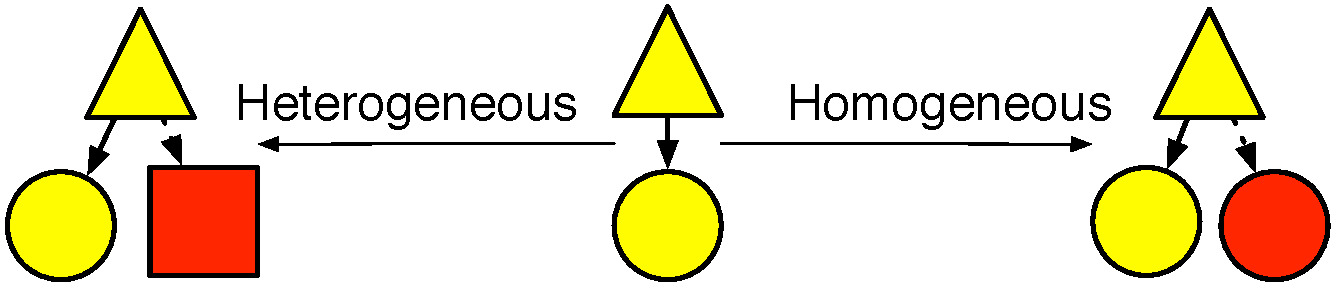
\epsfig{file=parameters/figures/HC.pdf, width=4in}
\caption{Appending a generator to the hierarchy.
The generator TODO module may be homogenous or heterogenous relative to its peers.}
\label{fig:hc}
\end{figure}

\begin{figure}
\centering
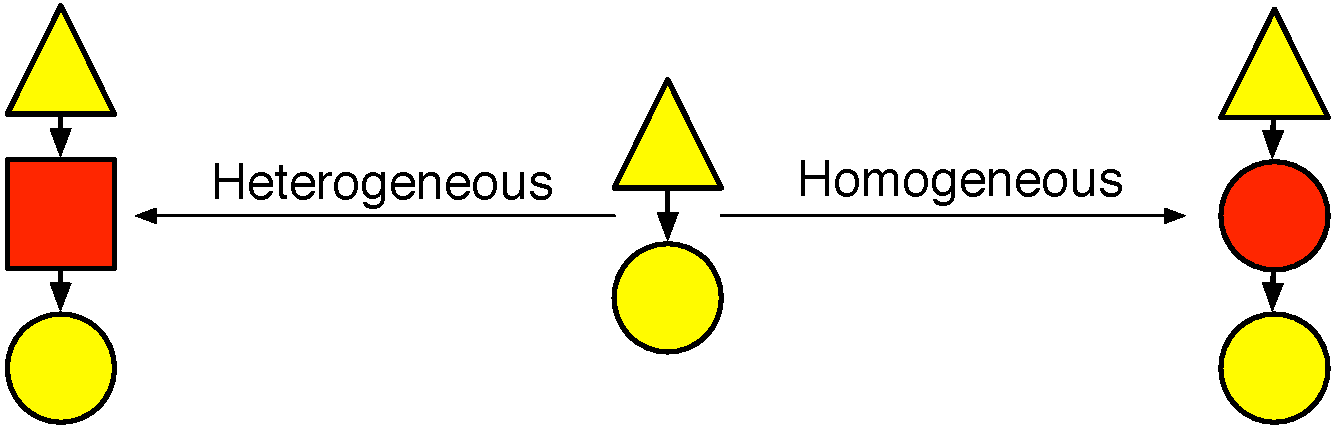
\epsfig{file=parameters/figures/VC.pdf, width=4in}
\caption{Inserting a module within the hierarchy.
The module may be homogenous or heterogenous relative to its child.}
\label{fig:vc}
\end{figure}

\begin{figure}
\centering
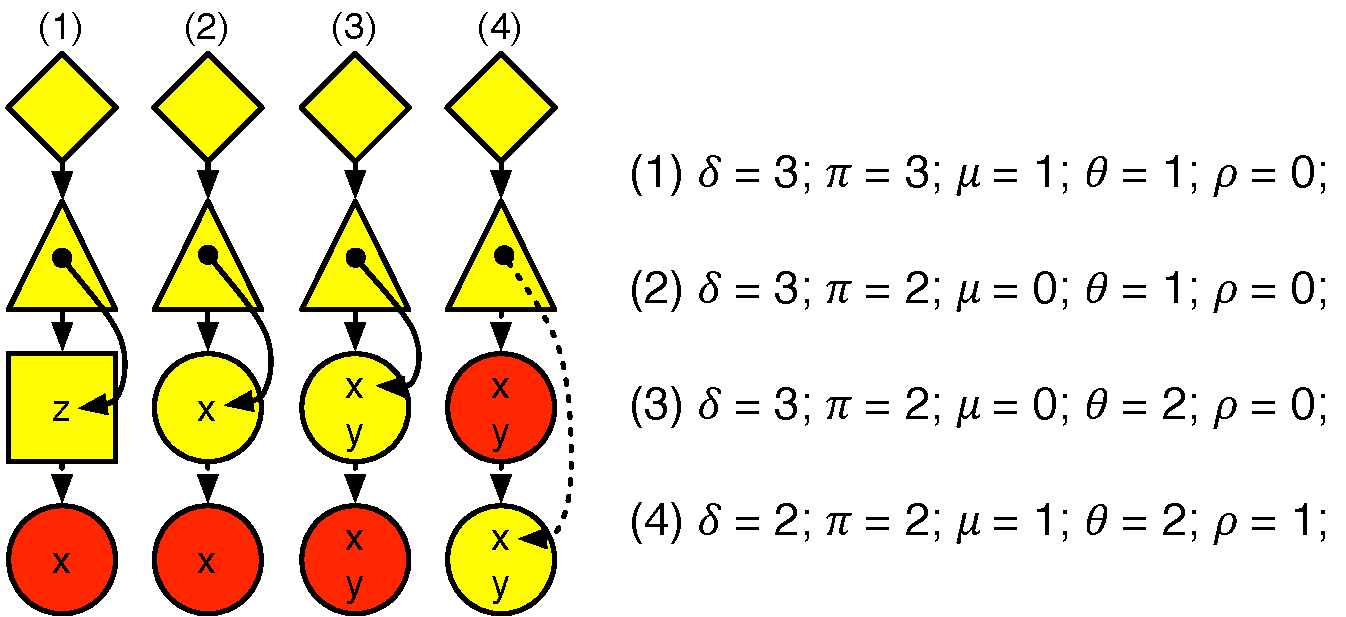
\epsfig{file=parameters/figures/CDSq.pdf, width = 5.5in}
\caption{(1)-(4) are example module hierarchies modifications. 
Module types are shapes, inserted/appended modules are red, and inter-module parameter references are curved arrows.
Nnote the broken reference in (4).}
\label{fig:attr}
\end{figure}

Section \ref{sec:tax} and Section \ref{sec:cde} used the case study of a tile generator to qualitatively contrast the efficacy of all five parameterization paradigms
at dealing with some specific modifications to the structure and hierarchy of hardware generators.
In this section we instead attempt to analytically describe the robustness of each paradigm to \textit{any possible set} of design modifications.
The results show that using CDEs \textit{always} results in a more robust design according to our metric,
but they also provide insight into when other paradigms could be equally appropriate.

As in the previous sections, we define robustness as the number of source code changes that cascade from making a modification to an existing design
consisting of a hierarchy of generators that elaborate hardware modules.
We generalize the initial modifications into one of two categories: appends or insertions.
An \emph{append} is when a new generator is incorporated as a leaf node whose instantiations do not affect the overall organization of the existing module hierarchy
(e.g. the addition of \code{PFPU} in Section \ref{sec:tax}).
In contrast, an \emph{insertion} is when a new generator is incorporated between an existing parent and child node in the hierarchy (e.g. the addition of \code{CacheWithPF}). 
Insertions change the overall structure of the module hierarchy.
Within each category, we differentiate betweeen whether the modification is homogenous or heterogenous, depending on whether the added module's type is the same as its sibling or child.
Figure \ref{fig:hc} illustrates these distinctions for appends and Figure \ref{fig:vc} does the same for insertions.

We assume all parameters added as part of a modification each require a unique value to be bound to their identifier the top-level of the module hierarchy.
These bindings must then be brought into the scope of the place where the parameters are evaluated.
Therefore, each original modification will trigger a varying number of scoping-related source code changes,
depending on both the existing module hierarchy as well as the parameterization paradigm being employed.

In order to characterize how many source code changes of each type will be required for each class of modification under each paramaterization paradigm,
we define the following attributes of a modification that introduces a new module, $M$, to the hierarchy:
\begin{itemize}%\itemsep1pt \parskip0pt \parsep0pt
\item $\delta$, the number of times any parent of $M$ is instantiated
\item $\pi$, $M$'s number of unique parent module declarations (that are not of type $M$)
\item $\mu$, whether $M$'s immediate parent has $M$'s type
\item $\theta$, the number of added parameters
\item $\rho$, the number of references to $M$'s child's parameters from any of $M$'s parents
\end{itemize}

Figure \ref{fig:attr} depicts four examples calculating these attributes for different module hierarchies
In (1), a new module with one parameter is heterogeneously appended to a 3-level hierarchy with each level being of a unique type.
In (2), a module with one parameter is homogenously appended to a 3-level hierarchy with two other types of modules.
In (3), a module with two parameters is homogenously appended to a 3-level hierarchy with two other types of modules.
In (4), a module with two parameters is homogenously inserted into a 3-level hierarchy with two other types of parameters.
In this case, $M$'s parent has a single reference to a parameter that is contained in $M$'s child.

Given these atrributes, we can calculate the number of top-level, non-local, and local changes per modification type under each paradigm.
Tables \ref{het:app}, \ref{hom:app}, \ref{het:ins}, and \ref{hom:ins} lay out the results.
Top-level changes are always equal to the number of parameters added by the modification ($\theta$).
Local changes consist of instantiating the new module and local manipulations of the module's parameter values.
Non-local changes include any other modifications, including parent instantiations, parent declarations, or modifying any parent's parameter object's instantiation/declaration.
Total changes are simply the sum of all LCs, NLCs, and TLCs.

Table \ref{het:app} shows the overhead of heterogenously appending a new module.
Under all paradigms, only a single LC is called for, because we simply can instantiate the new module.
The arg-list paradigm requires $(\delta+\pi)*\theta$ NLCs, because each of $\theta$ parameters must be threaded through the declarations ($pi$) and instantiations ($\delta$) of all of its parent modules in the hierarchy.
The flat-struct paradigm reduces this overhead to $\pi*\theta$ because the $\delta$ instantiations now refer to the struct instead of the individual parameters.
Surprisingly, nested-struct is almost equivalent to both environment passing schemes because $\mu$ is always either 0 or 1, depending on whether the immediate parent is of the same type as the appended module.

For homogenous appends (Table \ref{hom:app}), CDEs are slightly better than nested-structs, while regular environments perform poorly with $\theta$ additional source-code changes.
Table \ref{het:ins} shows that regular and CDE parameterization paradigms trigger zero NLCs,
but insertions into designs using argument lists, flat-structs, or nested-structs can trigger large numbers of NLCs depending on the module's depth, number of unique parents, or number of cross-module parameter references.

Homogeneous insertions, however, clearly show that CDEs are superior to all other paradigms (Table \ref{hom:ins}).
Regular environment passing is hindered by the additional $\theta$ renames, while nested-structs are limited by $\rho$, number of spanning parameter references. 
The single LC to CDEs is from modifying the parameter object's context prior to passing it to the inserted module, which is necessary to avoid the namespace renaming of regular environment passing.


Small designs with a shallow module hierarchy (e.g. a multiplier) are manageable with argument lists because the number of modification is limited. Any other design should move to a different paradigm.

Designs with shallow but wide hierarchies have few cross-module parameter references (e.g. networks) - insertions are rare and these designs are robust with nested-struct paradigms.

Deep hierarchical designs with minimal module reuse have heterogeneous insertions/appends and few parameter namespace collisions (e.g. a processor). These designs will remain robust with regular environment passing.

Complicated designs with deep hierarchies, significant module reuse, and many cross-module references have hetero- and homogeneous appends/insertions (e.g. SoC generator); these designs clearly benefit from CDEs.

%There is little benefit to using a context-dependent environment over a normal environment when most modifications to a design are only heterogenous. Unfortunately, more complicated designs often have homogeneous structures and, in this case, context-dependent environments are significantly superior. Use CHISEL because we've implemented context-dependent environments!!

\begin{table}
\centering
\begin{tabular*}{0.45\textwidth}{lccl}
\toprule
Paradigm    & LC & NLC & Total Changes\\
\midrule
arg-lists      &  1 & $(\delta+\pi)*\theta$ & $1+\theta*(\delta+\pi+1)$  \\
flat-struct  &  1 & $\pi*\theta$ &  1+$\theta$*($\pi$+1)  \\
nested-struct    &  1 & $\mu$ &  $1+\theta+\mu$  \\
regular-env    &  1 & 0 & $1+\theta$ \\
cde &  1 & 0 & $1+\theta$  \\
\bottomrule
\end{tabular*}
\caption{Appending a heterogenous module.}
\label{het:app}
\end{table}

\begin{table}
\centering
\begin{tabular*}{0.45\textwidth}{lccl}
\toprule
Paradigm    & LC & NLC &Total Changes\\
\midrule
arg-lists      &  1 & ($\delta$+$\pi$)*$\theta$ & 1+$\theta$*($\delta$+$\pi$+1)  \\
flat-struct  &  1 & $\pi$*$\theta$ & 1+$\theta$*($\pi$+1)  \\
nested-struct    &  1 & $\mu$ & 1+$\theta$+$\mu$  \\
regular-env    &  1+$\theta$ & 0 & 1+$\theta$*2 \\
cde &  2 & 0 & 2+$\theta$  \\
\bottomrule
\end{tabular*}
\caption{Appending a homogenous module.}
\label{hom:app}
\end{table}

\begin{table}
\centering
\begin{tabular*}{0.45\textwidth}{lccl}
\toprule
Paradigm    & LC & NLC & Total Changes\\
\midrule
arg-lists      &  1 & ($\delta$+$\pi$)*$\theta$ & 1+$\theta$*($\delta$+$\pi$+1)  \\
flat-struct  &  1 & $\pi$*$\theta$ & 1+$\theta$*($\pi$+1)  \\
nested-struct    &  1 & $\rho$+$\mu$ & 1+$\theta$+$\rho$+$\mu$  \\
regular-env    &  1 & 0&1+$\theta$ \\
cde &  1 & 0 & 1+$\theta$  \\
\bottomrule
\end{tabular*}
\caption{Inserting a heterogenous module.}
\label{het:ins}
\end{table}

\begin{table}
\centering
\begin{tabular*}{0.45\textwidth}{lccl}
\toprule
Paradigm    & LC & NLC & Total Changes\\
\midrule
arg-lists      &  1 & ($\delta$+$\pi$)*$\theta$& 1+$\theta$*($\delta$+$\pi$+1)  \\
flat-struct  &  1 & $\pi$*$\theta$ & 1+$\theta$*($\pi$+1)  \\
nested-struct    &  1 & $\rho$+$\mu$ & 1+$\theta$+$\rho$+$\mu$  \\
regular-env    &  1+$\theta$ & 0 & 1+$\theta$*2 \\
cde &  2 & 0 & 2+$\theta$  \\
\bottomrule
\end{tabular*}
\caption{Inserting a homogenous module.}
\label{hom:ins}
\end{table}


\section{Implementation of CDEs in Scala}
\label{sec:impl}

We augmented Chisel by leveraging its host language, Scala, to enable any Chisel design to use CDEs. 

At a high level, CDE values are not constant; they are functions whose arguments are 
(1) the query (\code{pname}) and 
(2) the CDE originally queried (\code{site}). 
The original CDE queried implicitly passes itself with every query. 
Ignoring the \code{site} argument turns the CDE into a regular environment; fancier parameter values based on querying \code{site} of existing parameters are now possible. 

\subsection{Environments as Partial Functions}

Lookup by \code{pname}.
Any type, e.g. matching on su

Return values.
Any type,
Field syntax for convenience.

Matching order.

Composablity.

\subsection{site}

parameters that depend on each other:
derivation, and
geography

\subsection{Constraints}

Operators on fields.

\subsection{External Interfaces}

Knobs: dumping and recording.

Constraints out: feed to solver.
Additional constraints in: for DSE.

Configurations as scala objects

\section{Parameterization Best Practices In Scala}

\subsection{Scala's Implicit Parameter Lists}

\subsection{Structs vs Fields}

\subsection{The Cake Pattern}

\subsection{Locations and Geography}

\subsection{Composing Configurations}

\subsection{Dealing with Heterogeneity}

\section{Discussion and Future Work}
\label{sec:con}

Relationship to HLS: Unlike high-level synthesis tools that transform abstract descriptions of a computation into gates, hardware generators are parameterized, programmatic descriptions of how to elaborate a templated RTL module hierarchy.

Runtime error handling: unbound parameters, dynamic typing, infinite recursion using site

Jackhammer and design space exploration

\section{Conclusion}
\label{sec:con}

We have presented a taxonomy of existing parameterization paradigms in HDLs and demonstrated that our context-dependent environments paradigm is provably more robust in the face of modification to any given design's module hierarchy. 

